\subsection{User Profiling}\label{subsec:userprofiling}

Creating user profiles is one the strengths Drive-LaB has. With a great set of metrics it is possible to differentiate between drivers, and create fairly accurate user profiles without compromising the users privacy. The entire concept of a user profile is relevant for this project as a possible connection to the insurance company. It is possible to evaluate the drivers insurance costs more precisely if the given user profile is accurate. However user profiles have to be accurate and portray the full picture when you are dealing with paying customers\citep{art:insurtelematics} -as they need an incentive to use the product. Throughout the section 2 different driver profiles will be reviewed and used to illustrate the differences. 

\paragraph{Score Percentages} are a great way to differentiate between drivers. The drivers will be referenced to as Driver 1 with an average tripscore percentage of 65,08\%, and Driver 2 with an average tripscore percentage of 39,07\%.

Besides the obvious difference in percentages, looking at where the drivers score their points shows differences. Figure \ref{fig:avgmetricper} and Figure \ref{fig:piecharts} shows a comparison between the two drivers, portrayed as a bar chart and a pie chart with the distribution of the tripscore based on metrics. Looking at Driver 1 is a lot of the score actually comes from accelerations at roughly 21\% increase, brakes at roughly 28\% and to some extend jerks at roughly 11\%. It is also worth mentioning that roadtypes actually scored negative on average. Looking at the pie chart, brakes is easily recognizable as the biggest sinner.

\begin{figure*}[tb]
\centering
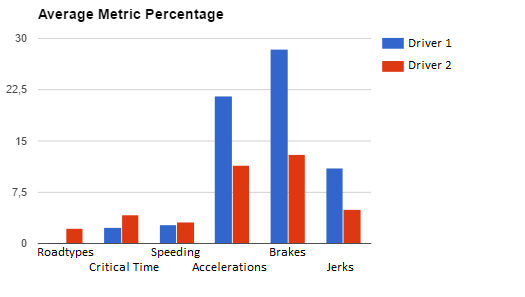
\includegraphics[width=0.465\textwidth]{Pictures/AverageMetricsPercentage}
\caption{A bar chart of the distribution of tripscore percentage by metrics for Driver 1 and Driver 2}
\label{fig:avgmetricper}
\end{figure*}

\begin{figure*}[tb]
\centering
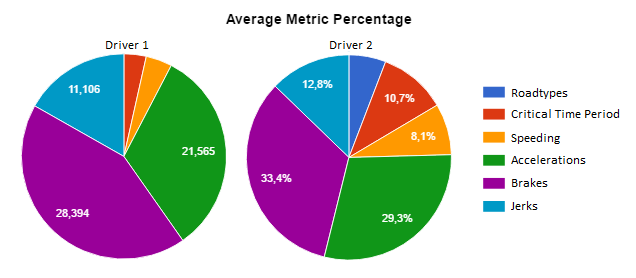
\includegraphics[width=0.95\textwidth]{Pictures/piecharts}
\caption{A bar chart of the distribution of tripscore percentage by metrics for Driver 1 and Driver 2}
\label{fig:piecharts}
\end{figure*}

Driver 2 has quite a different distribution than Driver 1, aside from a lower tripscore percentage in general. Accelerations and brakes clearly heavily influence the score in the system, however this driver have a significantly lower percentage in both of the metrics in the tripscore. This is noticeable in the pie chart which shows far less disparity between the metrics than the previous driver. 

\paragraph{Normalized Metrics} are the average metrics on a certain distance driven. For easy comparison the distance chosen is 1.000 meters. For instance looking at Driver 1 at Figure \ref{fig:avgmetricnorm}, Driver 1 has 6.84 points with jerks flagged per chosen distance. Looking at Driver 2 and comparing it to Driver 1, Driver 2 nearly has half the amount of accelerations, brakes and jerks per 1.000 meters. The only metric Driver 2 has more of per distance is speeding.

\begin{figure}[tb]
\centering
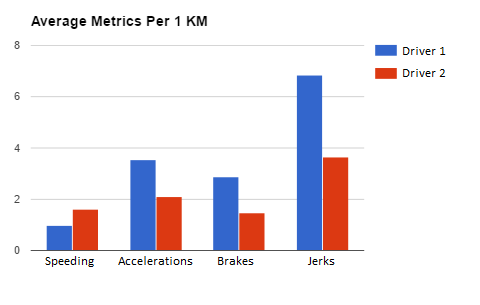
\includegraphics[width=0.465\textwidth]{Pictures/AverageMetricsNorm}
\caption{A bar chart of the metrics per 1.000 meters for Driver 1}
\label{fig:avgmetricnorm}
\end{figure}

\paragraph{Severity of Delinquencies} is one of the big tells when differentiating between drivers. It is noticeable when looking at Figure \ref{fig:car8intervals}, which represents Driver 1, there is a slight decline with a spike in the last interval. There might be several reasons as to why the last interval spike but the primary reason is the interval is everything above a threshold thus a much larger interval than the previous. Comparing Driver 1 to Driver 2, which is shown in Figure \ref{fig:car21intervals}, there is quite a different distribution.

\begin{figure*}[tb]
\centering
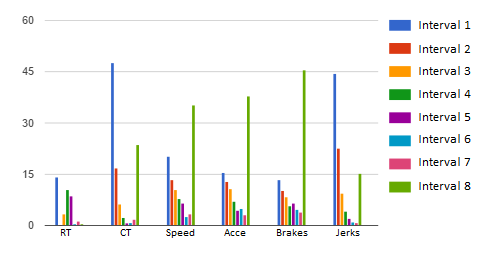
\includegraphics[width=0.95\textwidth]{Pictures/car8intervals}
\caption{A bar chart of the distribution of metrics within the intervals for Driver 1}
\label{fig:car8intervals}
\end{figure*}

\begin{figure*}[tb]
\centering
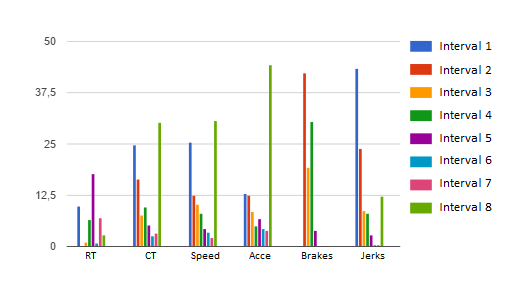
\includegraphics[width=0.95\textwidth]{Pictures/car21intervals}
\caption{A bar chart of the distribution of metrics within the intervals for Driver 2}
\label{fig:car21intervals}
\end{figure*}

It is possible to distinguish between drivers, and even more important, it is possible to create user profiles. Given a arbitrary trip it would be possible to draw similarities between the trip and the user profiles. From an insurance company point of view, it would be possible to access the risk of a given driver. As an example a driver with a higher amount of braking delinquencies and to a harder degree might have a higher risk of crashing -and get a more expensive insurance.